\setlength{\columnsep}{3pt}
\begin{flushleft}
		LVM are organized into: 
		\begin{itemize}
			\item Physical Volumes (PVs)
			\item Volume Groups (VGs)
			\item Logical Volumes (LVs)
		\end{itemize}
		
		\begin{figure}[h!]
			\centering
			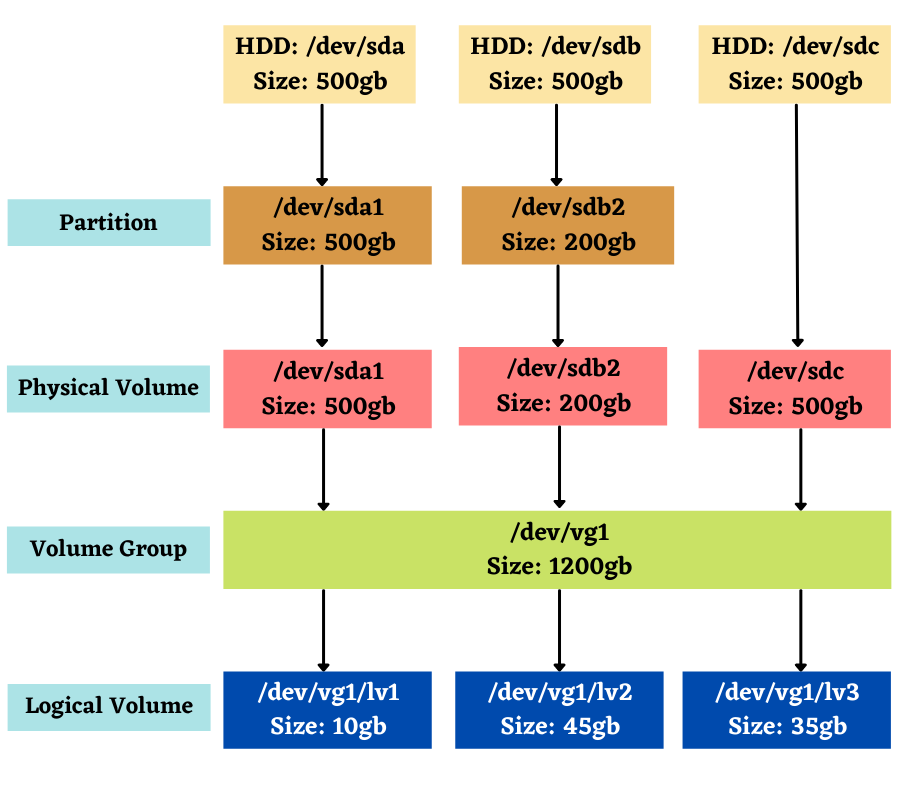
\includegraphics[scale=.6]{content/chapter9/images/lvm.png}
			\caption{LVM}
			\label{fig:lvm}
		\end{figure}
		
		\item Let's see each of these in detail.
	
	\newpage

	\paragraph{Physical Volumes (PVs)}
	\begin{itemize}
		\item Physical volumes are physical HDD or physical disk partitions (eg: /dev/sda or /dev/sdb1).
		\item In order to create LVM, you first need to create physical volumes out of HDD or partition to proceed.
	\end{itemize}

	
	\bigskip
	\bigskip
	\paragraph{Volume Goups (VGs)}
	\begin{itemize}
		\item A volume group is a collection of physical volumes.
		\item All volume groups would be created under \textbf{/dev} filesystem.
		\item \textbf{Eg: /dev/vg1}
	\end{itemize}

	\bigskip
	\bigskip
	\paragraph{Logical Volumes (LVs)}
	\begin{itemize}
		\item A volume group can be partitioned into logical volumes.
		\item Every logical volume can be located under it's VG.
		\item \textbf{Eg: /dev/vg1/lv1 , /dev/vg1/lv2 etc.}
	\end{itemize}

	\bigskip
	\bigskip
	\paragraph{Device Mapper}
	\begin{itemize}
		\item Device mapper is a Linux kernel module.
		\item Its job is to map devices names correctly to the physical devices.
		\item Eg: If the logical volume is named as \textbf{/dev/vg1/lv1}, device mapper will create mapping with name \textbf{/dev/mapper/vg1-lv1}.
	\end{itemize}

	

\end{flushleft}

\newpage

